\documentclass[a4paper, 12pt, twoside]{article}


%------------------------------------------------------------------------
%
% Author                :   arctan production
% Last modification     :   2023.1.12
%
%------------------------------------------------------------------------


%------ini
\usepackage[utf8]{inputenc}
\usepackage[T1]{fontenc}
\usepackage[french]{babel}
%\usepackage[english]{babel}


%------geometry
\usepackage[textheight=700pt, textwidth=500pt]{geometry}


%------color
\usepackage{xcolor}
\definecolor{0010A1}{HTML}{0010A1}
\definecolor{00f}{HTML}{0000ff}
\definecolor{0ff}{HTML}{00ffff}
\definecolor{656565}{HTML}{656565}

%\renewcommand{\emph}{\textcolor{0010A1}}
%\renewcommand{\em}{\color{0010A1}}

\newcommand{\Emph}{\textcolor{0010A1}}

\newcommand{\strong}[1]{\textcolor{0010A1}{\bf #1}}
\newcommand{\st}{\color{0010A1}\bf}


%------Code highlighting
%---listings
\usepackage{listings}

\definecolor{cbg}{HTML}{272822}
\definecolor{cfg}{HTML}{ececec}
\definecolor{ccomment}{HTML}{686c58}
\definecolor{ckw}{HTML}{f92672}
\definecolor{cstring}{HTML}{e6db72}
\definecolor{cstringlight}{HTML}{98980f}
\definecolor{lightwhite}{HTML}{fafafa}

\lstdefinestyle{DarkCodeStyle}{
    backgroundcolor=\color{cbg},
    commentstyle=\itshape\color{ccomment},
    keywordstyle=\color{ckw},
    numberstyle=\tiny\color{cbg},
    stringstyle=\color{cstring},
    basicstyle=\ttfamily\footnotesize\color{cfg},
    breakatwhitespace=false,
    breaklines=true,
    captionpos=b,
    keepspaces=true,
    numbers=left,
    numbersep=5pt,
    showspaces=false,
    showstringspaces=false,
    showtabs=false,
    tabsize=4,
    xleftmargin=\leftskip
}

\lstdefinestyle{LightCodeStyle}{
    backgroundcolor=\color{lightwhite},
    commentstyle=\itshape\color{ccomment},
    keywordstyle=\color{ckw},
    numberstyle=\tiny\color{cbg},
    stringstyle=\color{cstringlight},
    basicstyle=\ttfamily\footnotesize\color{cbg},
    breakatwhitespace=false,
    breaklines=true,
    captionpos=b,
    keepspaces=true,
    numbers=left,
    numbersep=10pt,
    showspaces=false,
    showstringspaces=false,
    showtabs=false,
    tabsize=4,
    frame=L,
    xleftmargin=\leftskip
}

%\lstset{style=DarkCodeStyle}
\lstset{style=LightCodeStyle}
%Usage : \begin{lstlisting}[language=Caml, xleftmargin=xpt] ... \end{lstlisting}


%---Algorithm
\usepackage[linesnumbered,ruled,vlined]{algorithm2e}
\SetKwInput{KwInput}{Input}
\SetKwInput{KwOutput}{Output}

\SetKwProg{Fn}{Function}{:}{}
\SetKw{KwPrint}{Print}

\newcommand\commfont[1]{\textit{\texttt{\textcolor{656565}{#1}}}}
\SetCommentSty{commfont}
\SetProgSty{texttt}
\SetArgSty{textnormal}
\SetFuncArgSty{textnormal}
%\SetProgArgSty{texttt}

\newenvironment{indalgo}[2][H]{
    \begin{algoBox}
        \begin{algorithm}[#1]
            \caption{#2}
}
{
        \end{algorithm}
    \end{algoBox}
}


%---tcolorbox
\usepackage[many]{tcolorbox}
\DeclareTColorBox{emphBox}{O{black}O{lightwhite}}{
    breakable,
    outer arc=0pt,
    arc=0pt,
    top=0pt,
    toprule=-.5pt,
    right=0pt,
    rightrule=-.5pt,
    bottom=0pt,
    bottomrule=-.5pt,
    colframe=#1,
    colback=#2,
    enlarge left by=10pt,
    width=\linewidth-\leftskip-10pt,
}

\DeclareTColorBox{algoBox}{O{black}O{lightwhite}}{
    breakable,
    arc=0pt,
    top=0pt,
    toprule=-.5pt,
    right=0pt,
    rightrule=-.5pt,
    bottom=0pt,
    bottomrule=-.5pt,
    left=0pt,
    leftrule=-.5pt,
    colframe=#1,
    colback=#2,
    width=\linewidth-\leftskip-10pt,
}


%-------make the table of content clickable
\usepackage{hyperref}
\hypersetup{
    colorlinks,
    citecolor=black,
    filecolor=black,
    linkcolor=black,
    urlcolor=black
}


%------pictures
\usepackage{graphicx}
%\usepackage{wrapfig}

\usepackage{tikz}
%\usetikzlibrary{babel}             %Uncomment this to use circuitikz
%\usetikzlibrary{shapes.geometric}  % To draw triangles in trees
%\usepackage{circuitikz}            %Electrical circuits drawing


%------tabular
%\usepackage{color}
%\usepackage{colortbl}
%\usepackage{multirow}


%------Mathpartir (inference rules)
\usepackage{mathpartir}


%------Physics
%---Packages
%\usepackage[version=4]{mhchem} %$\ce{NO4^2-}$

%---Commands
\newcommand{\link}[2]{\mathrm{#1} \! - \! \mathrm{#2}}
\newcommand{\pt}[1]{\cdot 10^{#1}} % Power of ten
\newcommand{\dt}[2][t]{\dfrac{\mathrm d #2}{\mathrm d #1}} % Derivative


%------math
%---Packages
%\usepackage{textcomp}
%\usepackage{amsmath}
\usepackage{amssymb}
\usepackage{mathtools} % For abs
\usepackage{stmaryrd} %for \llbracket and \rrbracket
\usepackage{mathrsfs} %for \mathscr{x} (different from \mathcal{x})

%---Commands
%-Sets
\newcommand{\N}{\mathbb{N}} %set N
\newcommand{\Z}{\mathbb{Z}} %set Z
\newcommand{\Q}{\mathbb{Q}} %set Q
\newcommand{\R}{\mathbb{R}} %set R
\newcommand{\C}{\mathbb{C}} %set C
\newcommand{\U}{\mathbb{U}} %set U
\newcommand{\seg}[2]{\left[ #1\ ;\ #2 \right]}
\newcommand{\nset}[2]{\left\llbracket #1\ ;\ #2 \right\rrbracket}

%-Exponantial / complexs
\newcommand{\e}{\mathrm{e}}
\newcommand{\cj}[1]{\overline{#1}} %overline for the conjugate.

%-Vectors
\newcommand{\vect}{\overrightarrow}
\newcommand{\veco}[3]{\displaystyle \vect{#1}\binom{#2}{#3}} %vector + coord

%-Limits
\newcommand{\lm}[2][{}]{\lim\limits_{\substack{#2 \\ #1}}} %$\lm{x \to a} f$ or $\lm[x < a]{x \to a} f$
\newcommand{\Lm}[3][{}]{\lm[#1]{#2} \left( #3 \right)} %$\Lm{x \to a}{f}$ or $\Lm[x < a]{x \to a}{f}$
\newcommand{\tendsto}[1]{\xrightarrow[#1]{}}

%-Integral
\newcommand{\dint}[4][x]{\displaystyle \int_{#2}^{#3} #4 \mathrm{d} #1} %$\dint{a}{b}{f(x)}$ or $\dint[t]{a}{b}{f(t)}$

%-left right
\newcommand{\lr}[1]{\left( #1 \right)}
\newcommand{\lrb}[1]{\left[ #1 \right]}
\newcommand{\lrbb}[1]{\left\llbracket #1 \right\rrbracket}
\newcommand{\set}[1]{\left\{ #1 \right\}}
\newcommand{\abs}[1]{\left\lvert #1 \right\rvert}
\newcommand{\ceil}[1]{\left\lceil #1 \right\rceil}
\newcommand{\floor}[1]{\left\lfloor #1 \right\rfloor}
\newcommand{\lrangle}[1]{\left\langle #1 \right\rangle}

%-Others
\newcommand{\para}{\ /\!/\ } %//
\newcommand{\ssi}{\ \Leftrightarrow \ }
\newcommand{\eqsys}[2]{\begin{cases} #1 \\ #2 \end{cases}}

\newcommand{\med}[2]{\mathrm{med} \left[ #1\ ;\ #2 \right]}  %$\med{A}{B} -> med[A ; B]$
\newcommand{\Circ}[2]{\mathscr{C}_{#1, #2}}

\renewcommand{\le}{\leqslant}
\renewcommand{\ge}{\geqslant}

\newcommand{\oboxed}[1]{\textcolor{0010A1}{\boxed{\textcolor{black}{#1}}}} %orange boxed

\newcommand{\rboxed}[1]{\begin{array}{|c} \hline #1 \\ \hline \end{array}} %boxed with right opened
\newcommand{\lboxed}[1]{\begin{array}{c|} \hline #1 \\ \hline \end{array}} %boxed with left opened

\newcommand{\orboxed}[1]{\textcolor{0010A1}{\rboxed{\textcolor{black}{#1}}}} %orange right boxed
\newcommand{\olboxed}[1]{\textcolor{0010A1}{\lboxed{\textcolor{black}{#1}}}} %orange left boxed


%------commands
%---to quote
\newcommand{\simplecit}[1]{\guillemotleft$\;$#1$\;$\guillemotright}
\newcommand{\cit}[1]{\simplecit{\textcolor{656565}{#1}}}
\newcommand{\quo}[1]{\cit{\it #1}}

%---to indent
\newcommand{\ind}[1][20pt]{\advance\leftskip + #1}
\newcommand{\deind}[1][20pt]{\advance\leftskip - #1}

%---to indent a text
\newcommand{\indented}[2][20pt]{\par \ind[#1] #2 \par \deind[#1]}
\newenvironment{indt}[2][20pt]{#2 \par \ind[#1]}{\par \deind} %Titled indented env

%---title
\newcommand{\thetitle}[2]{\begin{center}\textbf{{\LARGE \underline{\Emph{#1} :}} {\Large #2}}\end{center}}

%---Maths environments
%-Proofs
\newenvironment{proof}[1][{}]{\begin{indt}{$\square$ #1}}{$\blacksquare$ \end{indt}}

%-Maths parts (proposition, definition, ...)
\newenvironment{mathpart}[1]{\begin{indt}{\boxed{\text{\textbf{#1}}}}}{\end{indt}}
\newenvironment{mathbox}[1]{\boxed{\text{\textbf{#1}}}\begin{emphBox}}{\end{emphBox}}
\newenvironment{mathul}[1]{\begin{indt}{\underline{\textbf{#1}}}}{\end{indt}}

\newenvironment{theo}{\begin{mathpart}{Théorème}}{\end{mathpart}}
\newenvironment{Theo}{\begin{mathbox}{Théorème}}{\end{mathbox}}

\newenvironment{prop}{\begin{mathpart}{Proposition}}{\end{mathpart}}
\newenvironment{Prop}{\begin{mathbox}{Proposition}}{\end{mathbox}}
\newenvironment{props}{\begin{mathpart}{Propriétés}}{\end{mathpart}}

\newenvironment{defi}{\begin{mathpart}{Définition}}{\end{mathpart}}
\newenvironment{meth}{\begin{mathpart}{Méthode}}{\end{mathpart}}

\newenvironment{Rq}{\begin{mathul}{Remarque :}}{\end{mathul}}
\newenvironment{Rqs}{\begin{mathul}{Remarques :}}{\end{mathul}}

\newenvironment{Ex}{\begin{mathul}{Exemple :}}{\end{mathul}}
\newenvironment{Exs}{\begin{mathul}{Exemples :}}{\end{mathul}}


%------Sections
% To change section numbering :
% \renewcommand\thesection{\Roman{section}}
% \renewcommand\thesubsection{\arabic{subsection})}
% \renewcommand\thesubsubsection{\textit \alph{subsubsection})}

% To start numbering from 0
% \setcounter{section}{-1}


%------page style
\usepackage{fancyhdr}
\usepackage{lastpage}

\setlength{\headheight}{18pt}
\setlength{\footskip}{50pt}

\pagestyle{fancy}
\fancyhf{}
\fancyhead[LE, RO]{\textit{\textcolor{black}{\today}}}
\fancyhead[RE, LO]{\large{\textsl{\Emph{\texttt{\jobname}}}}}

\fancyfoot[RO, LE]{\textit{\texttt{\textcolor{black}{Page \thepage /}\pageref{LastPage}}}}
\fancyfoot[LO, RE]{
\includegraphics[scale=0.12]{arcln}}


%------init lengths
\setlength{\parindent}{0pt} %To avoid using \noindent everywhere.
\setlength{\parskip}{3pt}

% Mise en page française
\usepackage[utf8]{inputenc}
\usepackage[french]{babel}
\usepackage{geometry}

% Import d'images, couleurs
\usepackage{graphicx,color}

\usepackage{lipsum}

\newcommand{\hsp}{\hspace{20pt}}
\newcommand{\HRule}{\rule{\linewidth}{0.5mm}}

%---------------------------------Begin Document
\begin{document}

    
\begin{titlepage}
  \begin{sffamily}
  \begin{center}

  
    
\includegraphics[scale=0.3]{logo}~\\[1.5cm]

    \textsc{\LARGE EPITA Rennes}\\[0.5cm]

    % Titre
    \textsc{\Large CAHIER DES CHARGES DU PROJET S2}\\[1.5cm]

    \HRule \\[0.4cm]
     { \huge \bfseries  A Slime's Journey \\[0.4cm] }

    \HRule \\[2cm]
    
\includegraphics[scale=0.4]{arcln}
     \\[0.5cm]
    %\textsc{\Large ARCLN}\\[1.5cm]

    % Membres
    \begin{minipage}{0.4\textwidth}
      \begin{flushleft} \large
        Alexis LE GALL\\
        Enzo JUHEL\\
      \end{flushleft}
    \end{minipage}
    \begin{minipage}{0.4\textwidth}
      \begin{flushright} \large
        Maxime DOUILLARD\\
        Omid SHEIBANIFAR\\
      \end{flushright}
    \end{minipage}

    \vfill

  \end{center}
  \end{sffamily}
\end{titlepage}


    \tableofcontents
    \newpage

    \begin{indt}{\section{Introduction}}
        Dans ce cahier des charges nous aurons l'honneur de vous présenter le fruit de plusieurs années de recherches et probablement nos dernières , "A Slime's Journey" développé par la compagnie ARCLN. Ce jeu est un platformer 2D reliant histoire et énigmes et se déroulant dans un univers médiéval.

        Bien que nous soyons débutants dans le langage utilisé pour ce projet, nous avons tenté de trouver une idée originale en pensant aux jeux auxquels on a pu jouer auparavant, notre jeu se doit d'être digne d'intérêt et à la hauteur des capacités des membres du groupe et des attentes du jury.

        Le joueur prendra donc le contrôle d'un slime qui au contact de certains objets ou certaines matières pourra se transformer pour avancer dans le niveau, attention certains niveaux se termineront sur un combat de boss et il vous faudra redoubler de vigilance pour terrasser ceux ci. L'histoire se déroule de manière épisodique et un ou plusieurs nouveaux chapitres sortiront à chaque soutenance, cette manière de dérouler l'histoire permet d'implémenter une vraie expérience narrative sans forcément de cinématiques. Ce jeu pourra d'ailleurs être joué en coopération par le biais d'un mode multijoueur en ligne. D'un point de vue artistique, nous essaierons de rendre le jeu agréable à la vue et à l'ouïe, pour à la fois faire comprendre au joueur ce qu'il se passe, où il se trouve, quel est son but final et comprendre toute l'essence de l'histoire sans intervention scénaristique, tout en restant dans la lignée des platformers, c'est-à-dire rester à un certain niveau de difficulté quand même pour que le joueur aie une expérience complète. Une IA sera donc implémentée pour compliquer la tâche du joueur dans son aventure et proposer un véritable niveau de difficulté.
    \end{indt}

    \vspace{24pt}

    \begin{figure}[h!]
        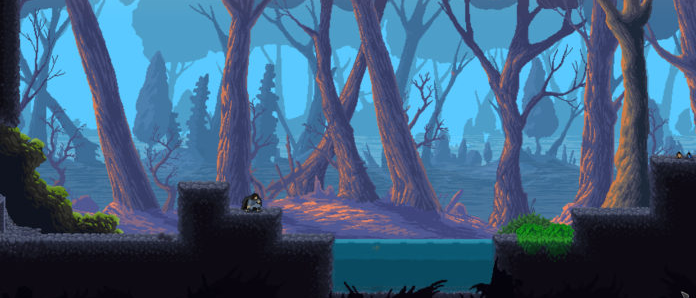
\includegraphics[width=\linewidth]{forest.png}
    \end{figure}
    
    \newpage

    \begin{indt}{\section{Plan}}
        \begin{indt}{\subsection{Origine et nature du sujet}}
            Ayant tous joué à des jeux de plateforme 2D durant notre enfance, tel que Super Mario Bros, il s'est avéré que c'était un type de jeu que nous connaissons tous très bien et avec de nombreuses références permettant une maîtrise du sujet. De plus, une créature fantastique simple mais au caractère divers, le slime, nous a paru une évidence d'où sa place de héros dans le jeu. Sans oublier que les power up, l'exploration, les combats $\&$ Co font partie de l'univers des jeux vidéo et permettent un niveau d'immersion supérieur. D'ailleurs un autre aspect des jeu vidéos sont leur univers, mieux ceux-ci sont construit, mieux le joueur va s'y retrouver immergé, pour cela, nous avons pris la liberté de construire un univers, un histoire et une intrigue se développant tout au long des différents chapitres et qui sera assimilable par le joueurs au travers le l'aspect d'exploration du jeu. C'est ainsi que nous avons donc décidé de partir ce ce modèle de jeu vidéo, un simple plateformer 2D renfermant une histoire profonde répartie sur plusieurs chapitres.
        \end{indt}

        \begin{indt}{\subsection{Inspirations}}
            Pour ce jeu nous nous sommes inspirés de jeux mainstreams comme mario ou kirby pour le coté gameplay , puis pour le coté lore et environnement nous nous somme inspiré du jeu limbo pour son côté très narratif sans forcément de cinématique. Pour les graphismes nous nous sommes tournés vers des dessins cartoons style cuphead.
        \end{indt}

        \begin{indt}{\subsection{Objet de l'étude}}
            D'une part, A slime's journey est un jeu fait pour le joueur. Un jeu de plateforme peut être joué de manières très diverses, les possibilités de gameplay sont infinies: du speedrun, finir le jeu à 100$\%$, finir le jeu avec un handicap. En résumé, chacun a la possibilité de jouer et apprécier le jeu à sa manière, le gameplay étant adapté au goût et au niveau de chacun. En effet, comme tout bon jeu de plateformes, des challenges seront disponibles pour les joueurs souhaitant relever un défi et terminer le jeu complètement. De plus, la difficulté du jeu sera adaptable afin que chacun puisse s'amuser. Pour ceux qui aiment jouer à plusieurs, le jeu sera disponible en coopération afin de vivre ou revivre l'aventure avec votre meilleur acolyte. D'autre part, cela constitue pour les développeurs un vrai défi créatif et enrichissant que ce soit en termes de level design, de coopération et de développement de projet.Ce projet permet à la fois de développer des compétences théoriques et pratiques. Le développement d'un jeu est à la fois un expérience de créativité, d'inventivité mais surtout d'accomplissement de projets. Il est primordial pour tout développeur de savoir délimiter et cadrer son projet de façon à le finir dans les temps tout en étant en concordance avec les attendus initiaux. Les difficultés ne relèvent pas que de l'aspect pratique mais aussi de la gestion du temps et du travail de chacun.

        \end{indt}

        \newpage

        \begin{indt}{\subsection{Etat de l'art}}
            Le premier jeu de type plate-formes est apparu en 1980 et porte le nom de Space Panic, édité par Universal, mais ce jeu ne permettait pas au joueur de sauter. En 1981, Nintendo sort le jeu Donkey Kong sur borne arcade, qui devient le premier jeu permettant au joueur de sauter par-dessus des obstacles et de franchir des précipices, devenant ainsi le premier jeu de plates-formes à proprement parler. A partir de 1982, de nombreux jeux de plates-formes voient le jour, comme Pitfall sur Atari 2600, Manic Miner, Jet Set Willy, Impossible Mission ou encore Prince of Persia. En 1985, Super Mario Bros. nait, il se vend à plus de 40 millions d'exemplaires et devient la norme des jeux de type plates-formes. En 1990, les jeux de plates-formes font leur apparition sous la forme de jeux 3D, comme Super Mario 64 en 1996. Ce type de jeu est toujours d'actualité, en effet, de nombreux jeux sortent encore, comme Super Meat Boy en 2010, de nouveaux jeux de la série Super Mario Bros, et bien d'autres.
        \end{indt}

        \begin{indt}{\subsection{Découpage du projet}}
            Un projet d'une telle ampleur nécessite une organisation sans faille afin de pouvoir tenir ces deadlines et garder un rythme de travail constant. C'est pourquoi, le développement se partage entre 3 aspects intimement liés, la communication, le management et le design. Le premier reflétant les échanges extérieurs des nouveautés, géré par Alexis et Maxime , que ce soit par la réalisation de trailers sur Youtube ou des annonces sur divers réseaux sociaux. Avec Enzo à la rédaction des différents documents à réaliser au cours du semestre. Ensuite, la supervision de l'équipe, réalisée à l'aide de Alexis, consiste à la prise de décisions, notamment lors de la réalisation de deadlines, répartition des tâches, etc. Enfin, la dernière section, et pas des moindres puisqu'il s'agit d'un point clé du développement, est régie par toute l'équipe, dont chaque membre ont leurs spécialités, tel que Maxime pour la modélisation des sprites sur Gimp, ou bien Enzo capable d'élaborer un level design dans Unity et encore, Omid pour le choix et la composition de musiques avec Audacity. En bref, voici un planning détaillé de répartition des tâches :
            \begin{center}
                \begin{tabular}{|c|c|c|c|c|}
                    \hline
                    & Alexis & Enzo & Maxime & Omid
                    \\
                    \hline
                    Développement & Participant & Participant & Responsable & Suppléant
                    \\
                    \hline
                    Communication & Suppléant & & Responsable &
                    \\
                    \hline
                    Design & & Responsable & Suppléant &
                    \\
                    \hline
                    Audio & Suppléant & & & Responsable
                    \\
                    \hline
                    IA & Responsable & & & Suppléant
                    \\
                    \hline
                    Réseau & Responsable & Suppléant & Participant & Participant
                    \\
                    \hline
                    Rédaction & Participant & Responsable & Participant & Suppléant
                    \\
                    \hline
                \end{tabular}
            \end{center}
        
        \end{indt}

    \end{indt}

    \vspace{12pt}

    \newpage

    \begin{indt}{\section{Structure}}
        \begin{indt}{\subsection{Fonctionnel}}
            La réalisation du projet jeu vidéo, se fera par chapitres, chacun délivrant une portion de l'histoire avec ces niveaux dédiés, dont le premier mettra en avant un tutoriel et une partie exploration. L'objectif est que la difficulté à chaque nouvelle sortie soit en adéquation avec l'expérience du joueur au sain du jeu, c'est pour cela que les premiers niveau sont plus orienté vers l'exploration, la découverte et la compréhension de l'univers dans lequel le héros se trouve, tandis qu'en s'approchant de la fin, se seront plutôt l'agilité et le combat qui seront de mise. Un autre aspect qui sera développé tout au long des différents rendus sont les power up, comme dit précédemment, le slime peut changer de forme selon l'environnement dans lequel il se trouve, lui donnant donc de nouvelles capacités offrant ainsi une diversité d'actions. Ainsi, l'implémentation des notions de vies et de boss de fin de chapitre permettent d'évaluer les capacité du joueurs, car ceux ayant prix le temps de garder la forme du slime la plus adéquate à la fin et n'ayant pas perdu de vies seront avantagé pour compléter le chapitre en question. Sans oublier que la coopération avec le joueur rejoignant la partie aide grandement l'avancée de la partie.

            Pour ce qui est du contenu en dehors du jeu lui-même, chaque chapitre aura le droit à un post sur Internet, que ce soit par un trailer Youtube, une annonce sur le Discord ou Instagram de l'équipe.
        \end{indt} 

        \begin{indt}{\subsection{Technologies et méthodologies}}
            Pour ce qui est du contenu en dehors du jeu lui-même, en plus du détail complet des nouveautés disponibles sur le site web officiel, chaque chapitre aura le droit à un post sur Internet, que ce soit par un trailer Youtube, une annonce sur le Discord ou Instagram de l'équipe.
        \end{indt} 

        \begin{indt}{\subsection{Opérationnel}}
            Cependant un tel jeu à des coûts monétaires, car chaque membre du groupe paye un logement sur Rennes, c'est pourquoi il faut comptabiliser le coût de repas quotidiens, loyer, factures d'électricité, d'eau, etc. Le tout sur 6 mois, bien qu'il soit possible de limiter ces dépenses en travaillant essentiellement sur le Campus, limitant ainsi le coût de l'électricité nécessaire au fonctionnement de nos pc, ainsi que l'eau, mise à disposition via la fontaine du rez-de-chaussée. C'est pourquoi, pour contrer autant de frais, le jeu sortira sous forme épisodique dont chaque nouvel épisode sera payant.
        \end{indt} 
    \end{indt}

    \newpage

    \begin{indt}{\section{Présentation}}
        \begin{indt}{\subsection{Scénario}}
            Le ou les joueurs incarnent un slime, une créature imaginaire avec des propriétés relevant de la magie. Le jeu vidéo A slime's journey nous permet de nous mettre dans la peau d'un slime, et, de découvrir un monde fantastique, remplis de mystères à élucider, de dangers à surmonter, comme des monstres, des précipices, et même des vices venant d'autres personnages. De plus, le jeu permettra aux joueurs de découvrir par eux-même les secrets du royaume, en passant par ses décors et ses habitants, le tout accompagné de musique, permettant une immersion totale. Au fur et à mesure de cette épopée, les joueurs devront rejoindre le château du roi de ce royaume, en traversant pour cela tout le royaume.
        \end{indt}
        
        \begin{indt}{\subsection{Gameplay}}
            Le jeu sera composé de deux phases, la sélection de niveau et la réalisation du niveau. Lors de la sélection du niveau, le jeu aura une vue de ¾, nous permettant de nous déplacer dans un monde restreint et de résoudre certaines énigmes. Lors de la réalisation du niveau, le jeu sera en 2D, vue de côté, comme la majorité des jeux de plateformes. Les joueurs pourront acquérir temporairement différentes capacités suivant la surface sur laquelle ils se trouvent, leur permettant ainsi de surmonter certains obstacles, ou d'esquiver des ennemis. Par exemple, lorsqu'un joueur se trouve sur une montagne, son slime prendra la forme d'un pique afin de se planter dans la montagne, lui donnant ainsi la possibilité de grimper à la montagne. Enfin, les joueurs pourront vaincre des monstres se trouvant sur leur passage à l'aide d'équipement ramassé au préalable durant les précédents niveaux, ou à l'aide de leurs capacités temporaires. Ce jeu est un jeu de plateformes, par conséquent, le fait de tomber dans le vide fait instantanément. Le fait de mourir, que ce soit en tombant ou en trépassant face à un monstre, le joueur perd une vie si il est en coopération et doit recommencer le niveau si il joue en solo, en coopération, si les deux joueurs meurent simultanément, le niveau devra également recommencer. A slime's journey comporte différents niveaux de difficultés, modifiant l'équipement obtenable, la quantité de vie des joueurs et des monstres, ainsi que les dégâts de ces derniers. Les ennemis seront gérés par des IAs différentes suivant la difficultées choisie. Il existe différents types d'items permettant de devenir plus résistants, avoir une meilleure portée d'attaque, de meilleurs dégâts, afin de vaincre de nouveaux ennemis de plus en plus coriaces. Les ennemis rencontrés au fur et à mesure de l'aventure dépendent de l'environnement du niveau, et permettent aux joueurs d'obtenir de l'équipement adapté à cet environnement.
        \end{indt}
    \end{indt}

    \begin{indt}{\section{Avancement du projet}}
        \begin{center}
            \begin{tabular}{|c|c|c|c|}
                \hline
                & Première Soutenance & Deuxième soutenance & Troisième soutenance
                \\
                \hline
                Développement & $33\%$ & $66\%$ & $100\%$
                \\
                \hline
                Communication & $33\%$ & $66\%$ & $100\%$
                \\
                \hline
                Design & $50\%$ & $75\%$ & $100\%$
                \\
                \hline
                Audio & $50\%$ & $75\%$ & $100\%$
                \\
                \hline
                IA & $50\%$ & $75\%$ & $100\%$
                \\
                \hline
                Réseau & $100\%$ & $100\%$ & $100\%$
                \\
                \hline
                Rédaction & $33\%$ & $66\%$ & $100\%$
                \\
                \hline
            \end{tabular}
        \end{center}
    \end{indt}

\end{document}
%--------------------------------------------End
